\chapter{基底の取り換えと行列表示}
\lectureinfo{2015年7月15日 1限}

\section{連絡事項など}

\paragraph{レポート解答の返却返却}

7/22に回収した皆さんのレポートは、添削してアドミニストレーション棟のレポートボックスに入れています。各自受け取っていってください。なお答案は学生証番号順に並べているので、\textbf{自分のを持っていく際に順番を乱さないでください}。

なお、過去に提出された答案も一緒に返却しています。受け取りそびれた人は、持って行ってください。

\paragraph{記法について} 「基底の変換行列」の話を書いていて気づいたのですが、もしかしたら、このプリントと授業と、あるいは他の本とで記法が違う箇所があるかもしれません。時と場合によってどういう記法が便利かが違ってくるので、このような現象が起きえます。もし試験で解答する際に気になることがあったら「どういう記法を使っているか」が分かる答案を書きましょう。そうすれば誤解の余地はありません。

\paragraph{その他、試験に向けて}

質問がある人は、先生にメールを送っても、TAの穂坂 \texttt{hosaka@ms.u-tokyo.ac.jp} にメールを送っても構いません。可能な限り応対します。

授業範囲を理解するのに必要なことは、これまでのプリントで大体書いたつもりです。試験まで残り$2$日しかないので、あまり色々な事はできないと思いますが、ノートとプリントを参考にして勉強しましょう。がんばってください。

\section{線型写像の行列表示}

これは非常に大事な話なのですが、あまりできている人が多くなかったので、なるべく丁寧めに解説をします。

まずは、話の筋を言ってしまいます。$f\colon U\rightarrow V$を線型写像とします。このとき
\begin{itemize}
\item $U$と$V$は共に基底を入れることで、数ベクトル空間と同一視される
\item この同一視のもと、$f\colon U\rightarrow V$は数ベクトル空間の間の線型写像になるから、行列で表示される
\end{itemize}
というわけです。とにかく\textbf{線型写像は行列だと思える}という点が大事です。行列にさえしてしまえば、後は掃き出し法とか色々な道具で計算ができるのですから。

\subsection{基底の復習}

$V$を線型空間とします。$V$の元の列$(\bm{f}_1, \bm{f}_2, \ldots, \bm{f}_n)$が\textbf{$V$の基底}であるとは
\begin{itemize}
\item $\{\bm{f}_1, \bm{f}_2, \ldots, \bm{f}_n\}$は$V$を生成する
\item $\{\bm{f}_1, \bm{f}_2, \ldots, \bm{f}_n\}$は$1$次独立である
\end{itemize}
という$2$つの条件が満たされることでした。そして$\bm{v} \in V$に対し
\[
\bm{v} = x_1 \bm{f}_1 + x_2 \bm{f}_2 + \cdots + x_n \bm{f}_n
\]
と表したとき、基底の係数$x_1, \ldots, x_n$を並べてできる数ベクトル${}^t(x_1, \ldots, x_n)$を  (基底$(\bm{f}_1, \ldots, \bm{f}_n)$に関する) $\bm{v}$の\textbf{座標}あるいは\textbf{成分表示}といいます。

基底を特徴づける$2$つの条件が、それぞれ「全てのベクトルに座標が割り当てられること」「座標の割り当て方がただ$1$通りであること」を保証することは、既に\pageref{subsec:basis}ページで説明しました。

\paragraph{線型空間の同型} いま$\bm{f}_1, \ldots, \bm{f}_n$を$V$の基底として、線型写像$\varphi\colon\mathbb{R}^n\rightarrow V$を
\[
\varphi\left(
\begin{pmatrix}
x_1 \\
\vdots \\
x_n
\end{pmatrix}
\right)
:= x_1 \bm{f}_1 + \cdots + x_n \bm{f}_n
\]
と定めます。すると基底の定義から
\begin{itemize}
\item $\bm{f}_1, \ldots, \bm{f}_n$は$V$を生成するので、$\varphi$は全射
\item $\bm{f}_1, \ldots, \bm{f}_n$は$1$次独立なので$\Ker\varphi = \{\bm{0}\}$となり、$\varphi$は単射
\end{itemize}
です。これより$\varphi$は全単射となり、$\varphi$によって$\mathbb{R}^n$と$V$の元とが$1:1$に対応します。さらに$\varphi$は線型写像だから、$\mathbb{R}^n$での加法/スカラー倍の結果を$\varphi$で送ったものは、先にベクトルを$\varphi$で送ってから$V$の中で加法/スカラー倍した結果と一致します。だから\textbf{線型空間の構造まで込めて、$\varphi$で$\mathbb{R}^n$と$V$が同一視されます}。

そして見れば分かりますが、$\varphi$で${}^t(x_1, \ldots, x_n) \in \mathbb{R}^n$を写した先にあるのは、基底$(\bm{f}_1, \ldots, \bm{f}_n)$のもとで座標${}^t(x_1, \ldots, x_n)$に対応する点です。ですから$\varphi$は、\textbf{座標とベクトルとの対応を与える写像}だといえます。逆に線型空間の同型$\varphi\colon \mathbb{R}^n\rightarrow V$が与えられれば、$\bm{f}_1 := \varphi(\bm{e}_1), \ldots, \bm{f}_n := \varphi(\bm{e}_n)$は$V$の基底をなします。したがって\textbf{座標を入れることは、$\varphi\colon \mathbb{R}^n \rightarrow V$で線型空間を同一視すること}に他なりません。

もう一度同じ式を書きますが
\[
\varphi\left(
\begin{pmatrix}
x_1 \\
\vdots \\
x_n
\end{pmatrix}
\right)
:= x_1 \bm{f}_1 + \cdots + x_n \bm{f}_n
\]
によって、$V$のベクトルとその座標とが対応します。だからこの$\varphi$は「座標をベクトルに読み替えるときのおまじない」みたいなものです。逆に$\varphi^{-1}$がついてたら「ベクトルを基底で展開した係数を拾い、対応する座標に読み替える」という意味になります。一度理解してしまえば大したことはないので、記号に慣れてください。

いっそ「線型空間に基底を入れちゃったら、もう$x_1\bm{f}_1 + \cdots + x_n\bm{f}_n$のことを${}^t(x_1, \ldots, x_n)$と書いていいじゃん」と思わなくもないし、実際に慣れてくるとそうすることも多いのですが、一方で「同一視のしかた」に気を配るのも数学の習わしです。今のうちは座標を考えるとき、きちんと$\varphi\bigl({}^t(x_1, \ldots, x_n)\bigr)$と書きましょう。

\subsection{線型写像の行列表示}

ここで$U, V$を線型空間とし、$f\colon U\rightarrow V$を線型写像とします。$(\bm{f}_1, \ldots, \bm{f}_n)$を$U$の基底、$(\bm{g}_1, \ldots, \bm{g}_m)$を$V$の基底とします。そうすると座標による同一視$\varphi\colon \mathbb{R}^n\rightarrow U$, $\psi\colon\mathbb{R}^m\rightarrow V$が得られます。図式では
\[
\begin{tikzcd}
U \arrow{r}{f} & V \arrow{d}{\psi^{-1}} \\
\mathbb{R}^n \arrow{u}{\varphi} \arrow[dashed]{r} & \mathbb{R}^m
\end{tikzcd}
\]
という感じです。ですから写像の合成$\psi^{-1}\circ f\circ\varphi$によって、\textbf{元々は$U$から$V$への線型写像だった$f$を、座標の入った$\mathbb{R}^n$から$\mathbb{R}^m$への線型写像に読み替える}ことができます。これは行列に他なりません。基底を取ることで、線型写像は行列表示できるのです\footnote{なお$U = V$で$f\colon V \rightarrow V$のときは、ふつう定義域と値域で同じ基底を取ります。線型変換を考えるときに、わざわざ違う基底を持ってくる理由はないですので。}。

非常に易しい例として、問4を解いてみましょう。皆さんは複素平面のことを知っていますから、$\mathbb{R}^2$のベクトルと$\mathbb{C}$を同一視できるはずです。この同一視のもと、$\mathbb{C}$の元に対する操作をベクトルに対する操作と読み替えて、行列で表示してみます。

\paragraph{問4の解答} 実線型空間$\mathbb{C}$の基底として$\{1, i\}$を取り、$\mathbb{C}$と$\mathbb{R}^2$を同一視する。このとき同一視を与える写像$\varphi\colon \mathbb{R}^2 \rightarrow \mathbb{C}$は
\[
\begin{pmatrix}
a \\
b
\end{pmatrix}
\overset{\varphi^{-1}}{\underset{\varphi}{\leftrightarrows}} a\cdot 1 + b\cdot i
\]
である\footnote{右辺は単に$a + bi$と書いてよいのですが、基底を明示するため、ここでは敢えて$a\cdot 1 + b\cdot i$と書いています。}。

\noindent (1) 複素数$\alpha = a + bi \in \mathbb{C}$について、$\alpha$倍写像$f_{\alpha}\colon \mathbb{C}\rightarrow\mathbb{C}$を考える。このとき$z = x + yi$に対し$f_{\alpha}(z) = \alpha z = (ax - by) + (bx + ay)i$である。この式を同一視$\varphi\colon\mathbb{R}^2\rightarrow\mathbb{C}$を使って読み替えると
\[
\begin{pmatrix}
x \\
y
\end{pmatrix}
\xmapsto{\text{\hbox to 3zw{\hfil$\varphi$\hfil}}}
x\cdot 1 + y\cdot i
\xmapsto{\text{\hbox to 3zw{\hfil$f_{\alpha}$\hfil}}} (ax - by)\cdot 1 + (bx + ay) \cdot i
\xmapsto{\text{\hbox to 3zw{\hfil$\varphi^{-1}$\hfil}}}
\begin{pmatrix}
ax - by \\
bx + ay
\end{pmatrix}
=
\begin{pmatrix}
a & -b \\
b & a
\end{pmatrix}
\begin{pmatrix}
x \\
y
\end{pmatrix}
\]
となっている。よって$f_{\alpha}$の行列表示は
\[
\begin{pmatrix}
a & -b \\
b & a
\end{pmatrix}
\]
である。

\noindent (2) $\iota\colon\mathbb{C}\rightarrow\mathbb{C}$を複素共役を取る写像とする。このとき$\iota(x + yi) = x - yi$なので、同一視$\varphi\colon\mathbb{R}^2\rightarrow\mathbb{C}$で読み替えると
\[
\begin{pmatrix}
x \\
y
\end{pmatrix}
\xmapsto{\text{\hbox to 3zw{\hfil$\varphi$\hfil}}} x\cdot 1 + y\cdot i
\xmapsto{\text{\hbox to 3zw{\hfil$\iota$\hfil}}} x\cdot 1 - y\cdot i
\xmapsto{\text{\hbox to 3zw{\hfil$\varphi^{-1}$\hfil}}}
\begin{pmatrix}
x \\
-y
\end{pmatrix}
=
\begin{pmatrix}
1 & 0 \\
0 & -1
\end{pmatrix}
\begin{pmatrix}
x \\
y
\end{pmatrix}
\]
となっている。よって$\iota$の行列表示は
\[
\begin{pmatrix}
1 & 0 \\
0 & -1
\end{pmatrix}
\]
である。 \qed

\paragraph{行列表示の計算}

では一般の場合$f\colon U\rightarrow V$は、どのような行列で表現されるのでしょうか?それを追いかけるために、「行列を線型写像とみたとき、成分の意味は何か」を考えてみましょう。$(m, n)$型行列$A = (a_{ij}) \in \Mat_{m, n}(\mathbb{R})$を$\mathbb{R}^n$の標準基底に作用させると
\[
A\bm{e}_j = 
\bordermatrix{
& & & & \scalebox{0.8}{$j^{\text{th}}$} \cr
& a_{11} & a_{12} & \cdots & a_{1j} & \cdots & a_{1n} \cr
& a_{21} & a_{22} & \cdots & a_{2j} & \cdots & a_{2n} \cr
& \vdots & \vdots & & \vdots & & \vdots \cr
& a_{m1} & a_{m2} & \cdots & a_{mj} & \cdots & a_{mn}
}
\begin{pmatrix}
0 \\
\vdots \\
0 \\
1 \\
0 \\
\vdots \\
0
\end{pmatrix}
=
\begin{pmatrix}
a_{1j} \\
a_{2j} \\
\vdots \\
a_{mj}
\end{pmatrix}
\]
となっています。つまり行列$A$の$j$列目は「標準基底の$j$番目のベクトル$\bm{e}_j$を$A$で移した先の$A\bm{e}_j$を、成分で表示したもの」になっています。

一般の場合もこれを真似て、$U$の基底を$f$で写した後に、$V$の基底で表示してみましょう。$U$の基底$(\bm{f}_1, \ldots, \bm{f}_n)$のそれぞれに対し、$f(\bm{f}_i)$は$V$の基底$(\bm{g}_1, \ldots, \bm{g}_m)$の$1$次結合で表されるはずです。その式を
\begin{align*}
f(\bm{f}_1) &= a_{11}\bm{g}_1 + a_{21}\bm{g}_2 + \cdots + a_{m1}\bm{g}_m \\
f(\bm{f}_2) &= a_{12}\bm{g}_1 + a_{22}\bm{g}_2 + \cdots + a_{m2}\bm{g}_m \\
&\vdots \\
f(\bm{f}_n) &= a_{1n}\bm{g}_1 + a_{2n}\bm{g}_2 + \cdots + a_{mn}\bm{g}_m
\end{align*}
とおきます。これを使って$f$の行列表示を求めます。まず
\begin{align*}
\varphi
\left(
\begin{pmatrix}
x_1 \\
\vdots \\
x_n
\end{pmatrix}
\right)
= x_1 \bm{f}_1 + \cdots + x_n \bm{f}_n
\end{align*}
で、座標を$U$のベクトルに読み替えます。これに$f$を施すと
\begin{align*}
f\circ \varphi
\left(
\begin{pmatrix}
x_1 \\
\vdots \\
x_n
\end{pmatrix}
\right)
&= f(x_1 \bm{f}_1 + \cdots + x_n \bm{f}_n) = x_1 f(\bm{f}_1) + \cdots + x_n f(\bm{f}_n) \\
&= x_1 (a_{11}\bm{g}_1 + a_{21}\bm{g}_2 + \cdots + a_{m1}\bm{g}_m) + \cdots +
x_n(a_{1n}\bm{g}_1 + a_{2n}\bm{g}_2 + \cdots + a_{mn}\bm{g}_m) \\
&= (a_{11} x_1 + a_{12} x_2 + \cdots + a_{1n} x_n)\bm{g}_1 + \cdots + (a_{m1} x_1 + a_{m2} x_2 + \cdots + a_{mn} x_n)\bm{g}_m
\end{align*}
となります。そして、このベクトルに$\psi^{-1}$を当てると座標が取り出せるので
\begin{align*}
\psi^{-1} \circ f\circ \varphi
\left(
\begin{pmatrix}
x_1 \\
\vdots \\
x_n
\end{pmatrix}
\right)
&=\psi^{-1}\bigl((a_{11} x_1 + a_{12} x_2 + \cdots + a_{1n} x_n)\bm{g}_1 + \cdots + (a_{m1} x_1 + a_{m2} x_2 + \cdots + a_{mn} x_n)\bm{g}_m \bigr) \\
&= 
\begin{pmatrix}
a_{11} x_1 + a_{12} x_2 + \cdots + a_{1n} x_n \\
a_{21} x_1 + a_{22} x_2 + \cdots + a_{2n} x_n \\
\vdots \\
a_{m1} x_1 + a_{m2} x_2 + \cdots + a_{mn} x_n
\end{pmatrix}
=
\begin{pmatrix}
a_{11} & a_{12} & \cdots & a_{1n} \\
a_{21} & a_{22} & \cdots & a_{2n} \\
\vdots & \vdots & \ddots & \vdots \\
a_{m1} & a_{m2} & \cdots & a_{mn}
\end{pmatrix}
\begin{pmatrix}
x_1 \\
x_2 \\
\vdots \\
x_n
\end{pmatrix}
\end{align*}
となります。ですから$f$は、行列
\[
\begin{pmatrix}
a_{11} & a_{12} & \cdots & a_{1n} \\
a_{21} & a_{22} & \cdots & a_{2n} \\
\vdots & \vdots & \ddots & \vdots \\
a_{m1} & a_{m2} & \cdots & a_{mn}
\end{pmatrix}
\]
で表現されると分かります。

この式をもう一度よく見ると、$j$列目に並ぶ$a_{1j}, a_{2j}, \ldots, a_{mj}$の出所は$f(\bm{f}_j) = a_{1j} \bm{g}_1 + a_{2j} \bm{g}_2 + \cdots + a_{mj} \bm{g}_m$という式です。ですから$f$の行列表示では、\textbf{$j$番目の基底に$f$を施してできるベクトルの成分表示が$j$列目にくる}ということになります。さっき、行列の積を線型写像と思ったときの話と全く同じですね。

これを踏まえた上で、問2, 3も解いてみましょう。

\paragraph{問3, 2の解答} $n$次以下の多項式全体のなす線型空間$\mathbb{R}[x]_{<n}$を
\[
\varphi\colon \mathbb{R}^{n + 1} \rightarrow \mathbb{R}[x]_{<n}; \quad
\begin{pmatrix}
b_0 \\
b_1 \\
\vdots \\
b_n
\end{pmatrix}
\mapsto b_0 + b_1 x + \cdots + b_n x^n
\]
によって$\mathbb{R}^{n + 1}$と同一視する\footnote{ここで行っているのは「多項式の各項の\uline{係数を拾って}ベクトルを作る」操作であって、決して「項そのものを並べてベクトルを作る操作」ではありません。勘違いしている人が非常に多かったので、注意しておきます。}。

全ての自然数$k\in\mathbb{N}$に対し$Dx^k = kx^{k - 1}$である。よって同一視$\varphi$を使うと、$D$は
\[
\begin{pmatrix}
b_0 \\
b_1 \\
\vdots \\
b_{n - 1} \\
b_n
\end{pmatrix}
\xmapsto{\text{\hbox to 1.5zw{\hfil$\varphi$\hfil}}} b_0 + b_1 x + \cdots + b_n x^n
\xmapsto{\text{\hbox to 1.5zw{\hfil$D$\hfil}}} b_1 + 2b_2 x + \cdots + n b_n x^{n - 1}
\xmapsto{\text{\hbox to 2.5zw{\hfil$\varphi^{-1}$\hfil}}}
\begin{pmatrix}
b_1 \\
2b_2 \\
\vdots \\
n b_n \\
0
\end{pmatrix}
=
\begin{pmatrix}
0 & 1 \\
& 0 & 2 \\
& & \ddots & \ddots \\
& & & 0 & n \\
& & & & 0
\end{pmatrix}
\begin{pmatrix}
b_0 \\
b_1 \\
\vdots \\
b_{n - 1} \\
b_n
\end{pmatrix}
\]
と見えるので、$D$の行列表示は
\[
\varphi^{-1}\circ D \circ \varphi
=
\begin{pmatrix}
0 & 1 \\
& 0 & 2 \\
& & \ddots & \ddots \\
& & & 0 & n \\
& & & & 0
\end{pmatrix}
\]
となる。また二項定理より、全ての自然数$k\in\mathbb{N}$に対し
\[
T_a x^k = (x - a) ^k = (-a)^k + \binom{k}{1} (-a)^{k - 1} x + \cdots + \binom{k}{k - 1} (-a) x^{k - 1} + x^k
\]
が成り立つ\footnote{ここで$\binom{k}{l}$は、二項係数を表します。${}_k C_l$と全く同じ意味ですが、大学の教科書や洋書ではほとんど$\binom{k}{l}$という記号が使われます。}。これで基底の行先が分かったので、$x^k$と$\bm{e}_{k + 1} \in \mathbb{R}^{n + 1}$が対応することを踏まえて、$T_a$の行列表示が
\[
\varphi^{-1} \circ T_a \circ \varphi 
=
\begin{pmatrix}
1 & -a & a^2 & -a^3 & \cdots & (-a)^n \\
 & 1 & -2a & 3a^2 & \cdots & \binom{n}{1}(-a)^{n - 1} \\
 & & 1 & -3a & & \vdots \\
 & & & 1 & \ddots & \vdots \\
 & & & & \ddots & \binom{n}{n - 1}(-a) \\
 & & & & & 1
\end{pmatrix}
\]
と分かる。\qed

\paragraph{関係式の「表現」} 合成函数の微分法を知っていると、多項式$f(x) \in \mathbb{R}[x]$に対し$\bigl(f(x - \alpha)\bigr)' = f'(x - \alpha)$が成り立つと分かります。この式をいまの$T_a$と$D$を使って書くと
\[
D\bigl(T_a f(x)\bigr) = T_a\bigl( Df(x) \bigr)
\]
に他なりません。さらに少し書き換えると$(D T_a - T_a D)\bigl(f(x)\bigr) = 0$が全ての多項式$f(x) \in \mathbb{R}[x]$に対して成り立ちます。だから$\mathbb{R}[x]$上の線型写像として、$D T_a - T_a D = 0$が成り立ちます。

この事実を反映して、さっき僕たちが求めた行列表示も$D T_a - T_a D = 0$を満たすはずです。たとえば$n = 3$のとき、実際に計算をすると確かに
\[
\begin{pmatrix}
1 & -a & a^2 & -a^3 \\
& 1 & -2a & 3a^2 \\
& & 1 & -3a \\
& & & 1
\end{pmatrix}
\begin{pmatrix}
0 & 1 \\
& 0 & 2 \\
& & 0 & 3 \\
& & & 0
\end{pmatrix}
=
\begin{pmatrix}
0 & 1 & -2a & 3a^2 \\
0 & 0 & 2 & -6a \\
0 & 0 & 0 & 3 \\
0 & 0 & 0 & 0
\end{pmatrix}
=
\begin{pmatrix}
0 & 1 \\
& 0 & 2 \\
& & 0 & 3 \\
& & & 0
\end{pmatrix}
\begin{pmatrix}
1 & -a & a^2 & -a^3 \\
& 1 & -2a & 3a^2 \\
& & 1 & -3a \\
& & & 1
\end{pmatrix}
\]
となっています。$n$は何でも良いですから、$n$に応じて$D T_a - T_a D = 0$という式を様々なサイズの行列で表現できる、というわけです。その他$T_a T_b = T_{a + b} = T_b T_a$などの関係式も、同様に成り立っています。興味のある人は確かめてみてください。

そして今は「平行移動」と「微分」という操作が先に与えられていましたが、逆に$D T_a - T_a D$のような「関係式」だけを最初に取り出して、後から「どのように行列で表現できるか」を考えることもしばしばあります。このような分野は\textbf{表現論}\index{ひょうげんろん@表現論}と呼ばれ、現代数学の主たる分野の$1$つを形成しています。

\section{基底の変換}

線型空間にはいくつもの基底があるので、それに応じていくつもの座標があります。それらの座標がどう関係するのかを、調べてみましょう。

\subsection{基底の変換行列}

\paragraph{基底の変換} 線型空間$V$に$2$つの基底が与えられたとします。このとき$2$つの基底に応じて$2$つの座標が定まります。すると当然「$2$つの座標はどのように対応するのか」が問題になります。すなわち、座標による同一視$\varphi, \psi\colon\mathbb{R}^n\rightarrow V$が与えられたとき、図式
\[
\begin{tikzcd}
& V & \\
\mathbb{R}^n \arrow[dashed]{rr} \arrow{ur}{\varphi} & & \mathbb{R}^n \arrow{ul}[swap]{\psi}
\end{tikzcd}
\]
における点線の矢印$\psi^{-1}\circ\varphi$が座標変換を表していて、これを具体的に行列で表示したいのです。

恒等写像$\id\colon\mathbb{R}^n\rightarrow\mathbb{R}^n$を使って今の図式に手を加えると
\[
\begin{tikzcd}
V \arrow{r}{\psi^{-1}} & \mathbb{R}^n \arrow{d}{\id} \\
\mathbb{R}^n \arrow{u}{\varphi} \arrow[dashed]{r} & \mathbb{R}^n
\end{tikzcd}
\]
とも書けます。こうすると、さっき線型写像を行列表示したときの図式と同じになります。だから座標変換の話は、座標を与える写像$\psi$の逆写像$\psi^{-1}\colon V\rightarrow \mathbb{R}^n$を、$\varphi$の定める基底および$\mathbb{R}^n$に関して行列表示することだと言えます。そうすれば「基底の行先を見ればよい」という話が自ずと見えてきます\footnote{ただ、座標を変換する話と基底を変換する話を区別しないと混乱します。この点については、すぐ後ろで述べます。}。

いま$\varphi$が定める基底を$(\bm{f}_1, \ldots, \bm{f}_n)$とし、$\psi$が定める基底を$(\bm{g}_1, \ldots, \bm{g}_n)$とします。このどちらもが基底だから、それぞれの$\bm{g}_i$は
\begin{align*}
\bm{g}_1 &= a_{11} \bm{f}_1 + a_{21} \bm{f}_2 + \cdots + a_{n1} \bm{f}_n \\
\bm{g}_2 &= a_{12} \bm{f}_1 + a_{22} \bm{f}_2 + \cdots + a_{n2} \bm{f}_n \\
&\vdots \\
\bm{g}_n &= a_{1n} \bm{f}_1 + a_{2n} \bm{f}_2 + \cdots + a_{nn} \bm{f}_n
\end{align*}
とただ$1$通りに表せます。これを行列っぽい記号で書くと
\[
\begin{pmatrix}
\bm{g}_1 & \bm{g}_2 & \cdots & \bm{g}_n
\end{pmatrix}
=
\begin{pmatrix}
\bm{f}_1 & \bm{f}_2 & \cdots & \bm{f}_n
\end{pmatrix}
\begin{pmatrix}
a_{11} & a_{12} & \cdots & a_{1n} \\
a_{21} & a_{22} & \cdots & a_{2n} \\
\vdots & \vdots & \ddots & \vdots \\
a_{n1} & a_{n2} & \cdots & a_{nn} \\
\end{pmatrix}
\]
となります。ここに出てくる行列を\textbf{基底$(\bm{f}_1, \ldots, \bm{f}_n)$から基底$(\bm{g}_1, \ldots, \bm{g}_n)$への変換行列}といいます。

\paragraph{座標変換と基底変換}

少々こんがらがる話になるのですが、\textbf{基底の変換と座標の変換を混同してはいけません}。今から見るように、基底をある正則行列$A$で別の基底に変換すると、対応する座標は$A^{-1}$で変換されます。

これまで通り$(\bm{f}_1, \ldots, \bm{f}_n)$と$(\bm{g}_1, \ldots, \bm{g}_n)$を共に$V$の基底とし、その基底の変換行列を$A$とします。すなわち
\[
\begin{pmatrix}
\bm{g}_1 & \bm{g}_2 & \cdots & \bm{g}_n
\end{pmatrix}
=
\begin{pmatrix}
\bm{f}_1 & \bm{f}_2 & \cdots & \bm{f}_n
\end{pmatrix} A
\]
です。そして$(\bm{f}_1, \bm{f}_2, \ldots, \bm{f}_n)$に関するベクトル$\bm{v}$の座標表示が${}^t(x_1, x_2 ,\ldots, x_n)$だったとしましょう。このとき$\bm{v} = x_1 \bm{f}_1 + x_2 \bm{f}_2 + \cdots + x_n \bm{f}_n$となるわけですが、この式を行列の積っぽい記法で
\[
\bm{v} = x_1 \bm{f}_1 + x_2 \bm{f}_2 + \cdots + x_n \bm{f}_n
=
\begin{pmatrix}
\bm{f}_1 & \bm{f}_2 & \cdots & \bm{f}_n
\end{pmatrix}
\begin{pmatrix}
x_1 \\
x_2 \\
\vdots \\
x_n
\end{pmatrix}
\]
と書き直してみます。こうすると\textbf{基底と座標のペアによって、ベクトルが定まること}が見やすいデスネ。そして、この表示だと基底と座標の間に行列を挟み込めるので
\begin{align*}
\bm{v}
&= 
\begin{pmatrix}
\bm{f}_1 & \bm{f}_2 & \cdots & \bm{f}_n
\end{pmatrix}
\begin{pmatrix}
x_1 \\
x_2 \\
\vdots \\
x_n
\end{pmatrix}
=
\begin{pmatrix}
\bm{f}_1 & \bm{f}_2 & \cdots & \bm{f}_n
\end{pmatrix}
A\cdot A^{-1}
\begin{pmatrix}
x_1 \\
x_2 \\
\vdots \\
x_n
\end{pmatrix}
=
\begin{pmatrix}
\bm{g}_1 & \bm{g}_2 & \cdots & \bm{g}_n
\end{pmatrix}
\cdot A^{-1}
\begin{pmatrix}
x_1 \\
x_2 \\
\vdots \\
x_n
\end{pmatrix}
\end{align*}
という式変形ができます。これで座標の変換規則が分かります。基底$(\bm{f}_1, \ldots, \bm{f}_n)$から$(\bm{g}_1, \ldots, \bm{g}_n)$に対する変換行列が$A$で与えられるとき、基底$(\bm{f}_1, \ldots, \bm{f}_n)$での座標に$A^{-1}$をかけたものが基底$(\bm{g}_1, \ldots, \bm{g}_n)$での座標になります。\textbf{基底の変換の仕方と座標の変換の仕方は逆行列の関係にある}ので、混同しないよう気を付けてください。

\paragraph{問1の解答}
\noindent (1)
\[
(x - a) ^k = (-a)^k + \binom{k}{1} (-a)^{k - 1} x + \cdots + \binom{k}{k - 1} (-a) x^{k - 1} + x^k
\]
なので
\[
\begin{pmatrix}
1 & x - a & (x - a)^2 & \cdots & (x - a)^n
\end{pmatrix}
=
\begin{pmatrix}
1 & x & x^2 & \cdots & x^n
\end{pmatrix}
\begin{pmatrix}
1 & -a & a^2 & -a^3 & \cdots & (-a)^n \\
 & 1 & -2a & 3a^2 & \cdots & \binom{n}{1}(-a)^{n - 1} \\
 & & 1 & -3a & & \vdots \\
 & & & 1 & \ddots & \vdots \\
 & & & & \ddots & \binom{n}{n - 1}(-a) \\
 & & & & & 1
\end{pmatrix}
\]
で基底の変換行列が求まる。

\noindent (2) $x^k = \bigl((x - a) + a\bigr)^k$より、(1) の変換行列で$a$を$-a$に置き換えたものが求める行列である。すなわち
\[
\begin{pmatrix}
1 & x & x^2 & \cdots & x^n
\end{pmatrix}
=
\begin{pmatrix}
1 & x - a & (x - a)^2 & \cdots & (x - a)^n
\end{pmatrix}
\begin{pmatrix}
1 & a & a^2 & a^3 & \cdots & a^n \\
 & 1 & 2a & 3a^2 & \cdots & \binom{n}{1}a^{n - 1} \\
 & & 1 & 3a & & \vdots \\
 & & & 1 & \ddots & \vdots \\
 & & & & \ddots & \binom{n}{n - 1}a \\
 & & & & & 1
\end{pmatrix}
\]
である。 \qed

\paragraph{基底変換の合成} 基底の変換行列の話が分かってしまえば、基底の変換を$2$度行うのは簡単です。いま$V$を線型空間、$(\bm{f}_1, \ldots, \bm{f}_n)$, $(\bm{g}_1, \ldots, \bm{g}_n)$と$(\bm{h}_1, \ldots, \bm{h}_n)$とをそれぞれ$V$の基底とします。そして基底の変換行列が
\[
\begin{pmatrix}
\bm{g}_1 & \bm{g}_2 & \cdots & \bm{g}_n
\end{pmatrix}
=
\begin{pmatrix}
\bm{f}_1 & \bm{f}_2 & \cdots & \bm{f}_n
\end{pmatrix} A, \quad
\begin{pmatrix}
\bm{h}_1 & \bm{h}_2 & \cdots & \bm{h}_n
\end{pmatrix}
=
\begin{pmatrix}
\bm{g}_1 & \bm{g}_2 & \cdots & \bm{g}_n
\end{pmatrix} B
\]
で与えられていたとしましょう。このとき基底$(\bm{f}_1, \ldots, \bm{f}_n)$から基底$(\bm{h}_1, \ldots, \bm{h}_n)$への変換行列は、上に書いた式を代入すれば
\[
\begin{pmatrix}
\bm{h}_1 & \bm{h}_2 & \cdots & \bm{h}_n
\end{pmatrix}
=
\begin{pmatrix}
\bm{g}_1 & \bm{g}_2 & \cdots & \bm{g}_n
\end{pmatrix} B
=
\begin{pmatrix}
\bm{f}_1 & \bm{f}_2 & \cdots & \bm{f}_n
\end{pmatrix} AB
\]
より$AB$と求まります。

\paragraph{基底変換による行列表示の変化}

ここまでの話のまとめとして、「線型写像の行列表示が、基底の変換でどう影響を受けるか」を調べます。ちょっとセッティングがややこしいので、箇条書きでまとめておきます。
\begin{itemize}
\item $U, V$は線型空間で、$f\colon U\rightarrow V$は線型写像
\item $(\bm{f}_1, \bm{f}_2, \ldots, \bm{f}_n)$, $(\bm{f}'_1, \bm{f}'_2, \ldots, \bm{f}'_n)$は共に$U$の基底で、それぞれが線型空間の同一視$\varphi, \varphi'\colon \mathbb{R}^n \rightarrow U$を与える
\item $(\bm{g}_1, \bm{g}_2, \ldots, \bm{g}_m)$, $(\bm{g}'_1, \bm{g}'_2, \ldots, \bm{g}'_m)$は共に$V$の基底で、それぞれが線型空間の同一視$\psi, \psi'\colon \mathbb{R}^m \rightarrow V$を与える
\end{itemize}
このとき$f$について
\begin{itemize}
\item $U$の基底$(\bm{f}_1, \bm{f}_2, \ldots, \bm{f}_n)$と$V$の基底$(\bm{g}_1, \bm{g}_2, \ldots, \bm{g}_m)$に関する行列表示$A$
\item $U$の基底$(\bm{f}'_1, \bm{f}'_2, \ldots, \bm{f}'_n)$と$V$の基底$(\bm{g}'_1, \bm{g}'_2, \ldots, \bm{g}'_m)$に関する行列表示$B$
\end{itemize}
を考えます。すると、$2$つの図式
\[
\begin{tikzcd}
U \arrow{r}{f} & V \arrow{d}{\psi^{-1}} \\
\mathbb{R}^n \arrow{u}{\varphi} \arrow[dashed]{r}{A} & \mathbb{R}^m
\end{tikzcd}, \quad
\begin{tikzcd}
U \arrow{r}{f} & V \arrow{d}{(\psi')^{-1}} \\
\mathbb{R}^n \arrow{u}{\varphi'} \arrow[dashed]{r}{B} & \mathbb{R}^m
\end{tikzcd}
\]
ができます。続いて
\begin{itemize}
\item 基底$(\bm{f}_1, \bm{f}_2, \ldots, \bm{f}_n)$から基底$(\bm{f}'_1, \bm{f}'_2, \ldots, \bm{f}'_n)$への変換行列$P$
\item 基底$(\bm{g}_1, \bm{g}_2, \ldots, \bm{g}_m)$から$(\bm{g}'_1, \bm{g}'_2, \ldots, \bm{g}'_m)$への変換行列$Q$
\end{itemize}
を考えます。するとさらに$2$つ
\[
\begin{tikzcd}
& V & \\
\mathbb{R}^n \arrow{rr}{P^{-1}} \arrow{ur}{\varphi} & & \mathbb{R}^n \arrow{ul}[swap]{\varphi'}
\end{tikzcd}, \quad
\begin{tikzcd}
& V & \\
\mathbb{R}^m \arrow{rr}{Q^{-1}} \arrow{ur}{\psi} & & \mathbb{R}^m \arrow{ul}[swap]{\psi'}
\end{tikzcd}
\]
という図式ができます\footnote{この図式は「$2$通りに回れるところは、どっちを回っても同じ結果になる」という意味です。このような図式を\textbf{可換図式}といいます。}。こうしてできた$4$つの図式を合体させると、こうなります: 
\[
\begin{tikzcd}
\mathbb{R}^n \arrow{rrr}{A}\arrow{rd}{\varphi} \arrow{dd}[swap]{P^{-1}} & & & \mathbb{R}^m \arrow{dd}{Q^{-1}} \\
& U \arrow{r}{f} & V \arrow{ru}[swap]{\psi^{-1}} \arrow{rd}[swap]{(\psi')^{-1}} & \\
\mathbb{R}^n \arrow{rrr}[swap]{B} \arrow{ru}{\varphi'} & & & \mathbb{R}^m
\end{tikzcd}
\]
複数の回り方があるところは、どう回っても同じです。だから左下の$\mathbb{R}^n$から右下の$\mathbb{R}^m$への写像$B\colon\mathbb{R}^n\rightarrow\mathbb{R}^m$は、一旦$P\colon\mathbb{R}^n\rightarrow\mathbb{R}^n$で上に行き、そこから$A$で右上の$\mathbb{R}^m$に行き、さらに$Q^{-1}$で右下に移動するのと同じです。もうちょっとちゃんと書くと
\[
B = (\psi')^{-1}\circ f \circ \varphi' = (Q^{-1}\circ\psi^{-1})\circ f\circ (\varphi\circ P) = Q^{-1}\circ A \circ P
\]
という変形をやっています。上にある図式とにらめっこしながら、どういう経路をたどっているのか、一度追いかけてみてください。これで基底の変換に応じて、行列表示が$B = Q^{-1} A P$という公式で置き換わることが分かりました\footnote{この公式は重要ですが、式を丸覚えするのはやめた方がいいです。というのも「変換行列はどっち向きだっけ?」とかを思い出そうとすると、大体どこかでミスするからです。上に書いた図式を再現できるようになっておきましょう。}。

ちなみにこの図式は「座標変換で行列表示は色々変化するが、その中心にいるのは$f\colon U\rightarrow V$である」と言っているように見えます。特に$P$や$Q$として基本行列を持ってくると、$B$は$A$に行/列基本変形をした結果になります。僕たちは上手い基本変形で行列の像や核を求める計算をしましたが、それは「真ん中にいる$f$を色々な角度から眺めて、その性質を探ろうとしていた」と言うことができるのです。

\subsection{一般化された内積}

問5は、区間$[0, 2\pi]$の適当な値を代入したり、微分したりとかで解くことができます。ですが今回はちょっとやり方を変えて、積分を使って解いてみましょう。

\paragraph{問5の解答} $W$は$\{1, \cos x, \sin x, \cos 2x, \sin 2x\}$が張る空間である。この集合が$1$次独立であることを示して、$\dim W = 5$をいう。

\noindent \underline{step 1.}
まず、正の整数$m, n \in \mathbb{Z}_{>0}$に対し
\begin{align*}
\frac{1}{\pi}\int_0^{2\pi} \cos mx \cos nx \, dx &=
\frac{1}{\pi}\int_0^{2\pi} \sin mx \sin nx \, dx
= \delta_{mn} :=
\begin{cases}
1 & (m = n) \\
0 & (m \neq n)
\end{cases} \\
\frac{1}{\pi}\int_0^{2\pi} \cos mx \sin nx \, dx &= \frac{1}{\pi}\int_0^{2\pi} \cos mx \, dx = \frac{1}{\pi}\int_0^{2\pi} \sin mx \, dx = 0
\end{align*}
が成り立つ\footnote{ここで$\delta_{nm}$は、$n = m$なら$1$、そうでないなら$0$という意味です。この記号は「Kroneckerの$\delta$」と呼ばれ、たとえば単位行列を$I = (\delta_{ij})$と表したりするときに使います。}ことを確認しておく\footnote{この式は大学入試でも割とよく見かける式なので、証明は略します。三角函数の積和公式を使って変形した後、$m = n$かそうでないかに応じて愚直に積分すれば求まります。}。

\noindent \underline{step 2.} 次に$C^0\bigl([0, 2\pi]\bigr)$を、閉区間$[0, 2\pi]$上の連続函数全体の集合とする\footnote{しばしば$\mathbb{R}$上の連続函数のことを「$C^0$級函数」というので、その記法を使いました。}。$f, g \in C^0\bigl([0, 2\pi]\bigr)$に対し
\[
(f, g) := \frac{1}{\pi} \int_0^{2\pi} f(x) g(x) dx
\]
と定める。すると全ての$f_1, f_2, g \in C^0\bigl([0, 2\pi]\bigr)$と$\alpha, \beta\in\mathbb{R}$に対し
\begin{align*}
(\alpha f_1 + \beta f_2, g)
&=
\frac{1}{\pi} \int_0^{2\pi} \bigl(\alpha f_1(x) + \beta f_2(x)\bigr) g(x) dx
= \frac{\alpha}{\pi} \int_0^{2\pi} f_1(x) g(x) dx + \frac{\beta}{\pi} \int_0^{2\pi} f_2(x) g(x) dx \\
&= \alpha(f_1, g) + \beta(f_2, g)
\end{align*}
が成り立つ。つまり$g$を止めたとき、写像$f \mapsto (f, g)$は線型である。さらにこの記号を使うと、さっき示した三角函数の公式は
\[
(\cos mx , \cos nx ) = (\sin mx, \sin nx) = \delta_{mn},\quad (\cos mx, \sin nx) = 0
\]
と表せる。

\noindent \underline{step 3.} これで準備ができたので、$\{1, \cos x, \sin x, \cos 2x, \sin 2x\}$の$1$次独立性を示す。$f(x) := a + b\cos x + c \sin x + d \cos 2x + e \sin 2x \equiv 0$とおく。このとき任意の函数$g \in C^0\bigl([0, 2\pi]\bigr)$に対し$(f, g) = (0, g) = 0$が成り立つので
\begin{align*}
\begin{array}{l@{\,}l@{\,}l@{\,}l@{\,}l@{\,}l@{\,}l@{\,}l@{\,}l@{\,}l@{\,}l@{\,}l}
0 &= \bigl(f(x), 1 \bigr) &= a(1, 1) &+& b(\cos x, 1) &+& c (\sin x, 1) &+& d (\cos 2x, 1) &+& e (\sin 2x, 1) &= a \rule{0zw}{1.5zw}\\
0 &= \bigl(f(x), \cos x \bigr) &= a(1, \cos x) &+& b(\cos x, \cos x) &+& c (\sin x, \cos x) &+& d (\cos 2x, \cos x) &+& e (\sin 2x, \cos x) &= b \rule{0zw}{1.5zw}\\
0 &= \bigl(f(x), \sin x \bigr) &= a(1, \sin x) &+& b(\cos x, \sin x) &+& c (\sin x, \sin x) &+& d (\cos 2x, \sin x) &+& e (\sin 2x, \sin x) &= c \rule{0zw}{1.5zw}\\
0 &= \bigl(f(x), \cos 2x \bigr) &= a(1, \cos 2x) &+& b(\cos x, \cos 2x) &+& c (\sin x, \cos 2x) &+& d (\cos 2x, \cos 2x) &+& e (\sin 2x, \cos 2x) &= d \rule{0zw}{1.5zw}\\
0 &= \bigl(f(x), \sin 2x \bigr) &= a(1, \sin 2x) &+& b(\cos x, \sin 2x) &+& c (\sin x, \sin 2x) &+& d (\cos 2x, \sin 2x) &+& e (\sin 2x, \sin 2x) &= e \rule{0zw}{1.5zw}
\end{array}
\end{align*}
となる。これで$1$次独立性が言えた。\qed

\paragraph{Fourier級数展開} \label{paragraph:Fourier_series}

いまの証明からほとんど明らかですが、$\cos$や$\sin$の中に入るのは別に$x$や$2x$でなくとも構いません。積分を使って定義された$(f,g)$を使えば、$\{1, \cos x, \sin x, \cos 2x, \sin 2x, \cos 3x, \sin 3x,\ldots\}$は$1$次独立だと示せます\footnote{より正確には「この集合に含まれるどんな有限部分集合を持ってきても、その元たちが$1$次独立になる」という意味です。}。では、$C^0\bigl([0, 2\pi]\bigr)$の基底にはなるでしょうか?

この答えは、普通の基底の定義に照らせば``No''です。三角函数ではない函数はいくらでもあります。たとえば多項式がその典型的な例です。ですから$\{1, \cos x, \sin x, \cos 2x, \sin 2x, \cos 3x, \sin 3x, \ldots\}$の元を単純に足し算するだけでは、$C^0\bigl([0, 2\pi]\bigr)$の全ての元を作ることはとでもできません。ですが単純な足し算ではなく「無限和」、つまり函数の和の極限を考えれば、$C^0\bigl([0, 2\pi]\big)$の函数たちをいくらでも良く近似できることが知られています。たとえば直線$y = x$を区間$[-\pi, \pi]$で\footnote{計算の都合上、区間$[0, 2\pi]$を$-\pi$だけずらして$[-\pi, \pi]$上で考えます。元の区間$[0, 2\pi]$でも計算できるのですが、今回は$[-\pi, \pi]$の方が計算しやすかったのです。}近似する式は
\[
x = \sum_{m = 1}^{\infty} \sin mx \cdot \frac{1}{\pi} \int_{-\pi}^{\pi} t \sin mt\, dt = \sum_{m = 1}^{\infty} (-1)^{m + 1} \frac{2}{m} \sin mx
\]
です。問5を解くときに「$\bigl(f(x), \cos x\bigr)$がちょうど$f(x)$における$\cos x$の係数になる」などの事実を使いましたが、それと同じようにして、$x$を$\{1, \cos x, \sin x, \cos 2x, \sin 2x, \ldots\}$の「線型結合」で表したときの係数を、積分で取り出しています。途中までの和をグラフにしてみると、確かに近似になっていることが分かりますね。

\begin{figure}[h!tbp]
\centering
\subfigure[$m = 1$まで]{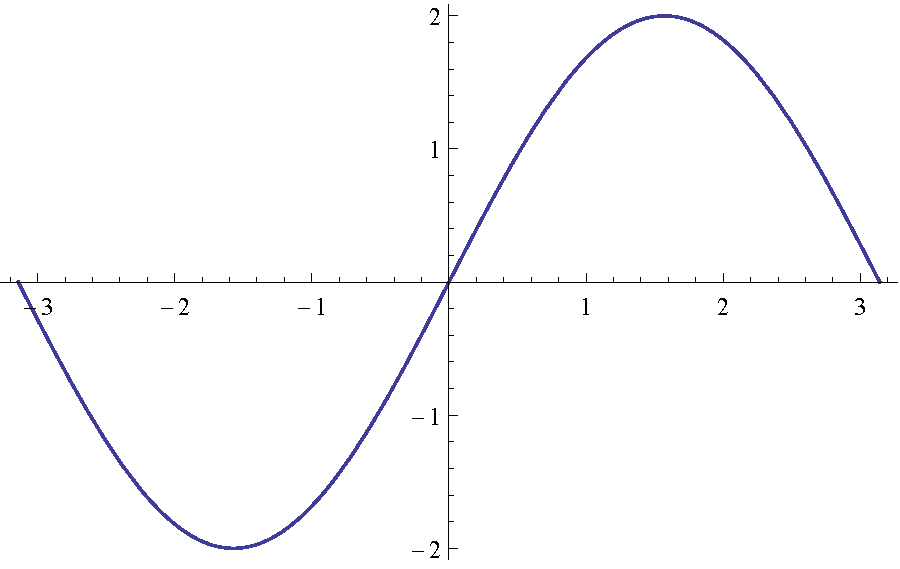
\includegraphics[width = .2\textwidth]{20150715-fig-Fourier1.pdf}} \raisebox{3zw}{$\longrightarrow$}
\subfigure[$m = 4$まで]{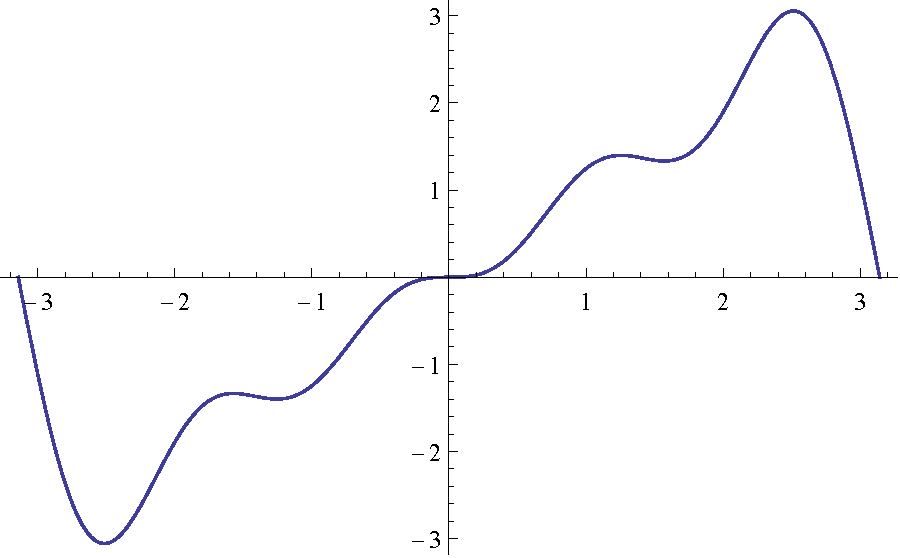
\includegraphics[width = .2\textwidth]{20150715-fig-Fourier2.pdf}} \raisebox{3zw}{$\longrightarrow$}
\subfigure[$m = 16$まで]{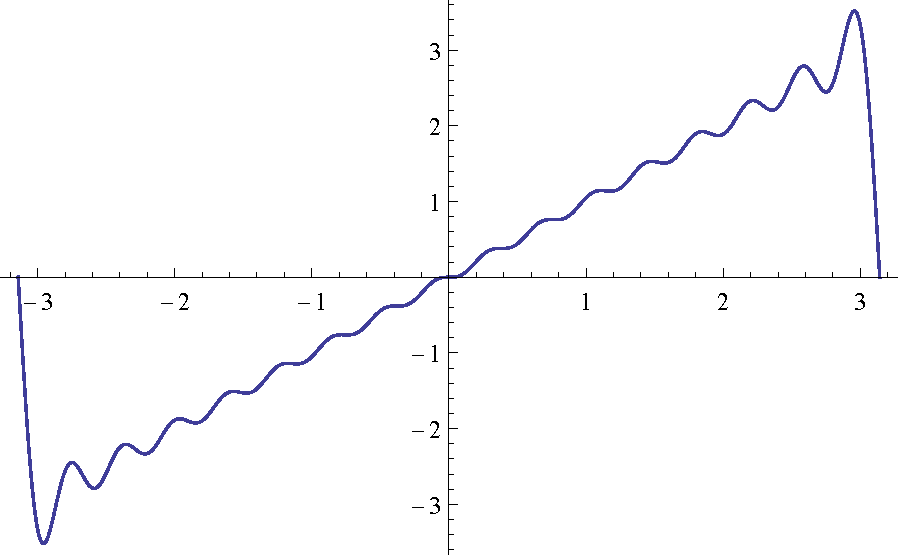
\includegraphics[width = .2\textwidth]{20150715-fig-Fourier3.pdf}} \raisebox{3zw}{$\longrightarrow$}
\subfigure[$m = 64$まで]{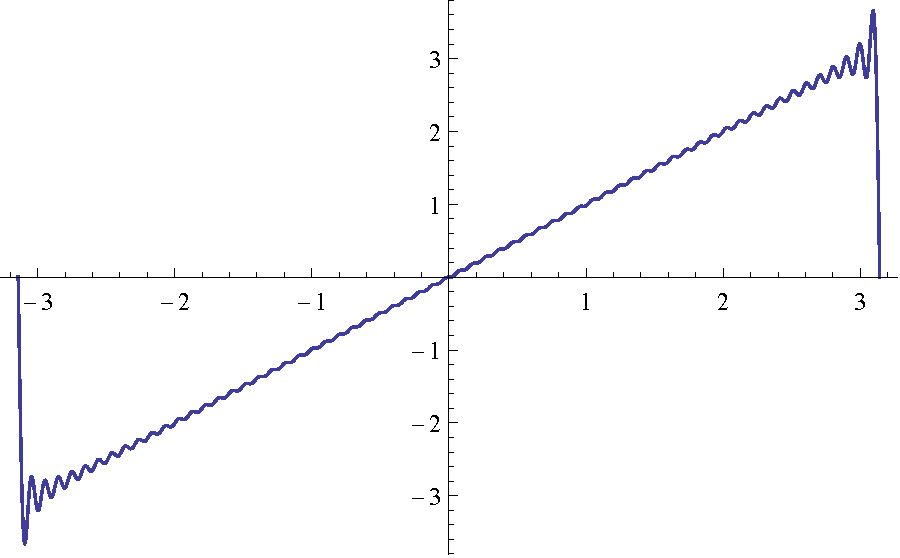
\includegraphics[width = .2\textwidth]{20150715-fig-Fourier4.pdf}}
\caption{閉区間$[-\pi, \pi]$における$y = x$のFourier級数展開の様子}
\end{figure}

このように、函数を$\{1, \cos mx, \sin mx \mid m\in\mathbb{Z}_{>0}\}$の無限級数で表すことを\textbf{Fourier級数展開}\index{Fourierきゅうすう@Fourier級数}といいます。音波や交流など「波」を扱う際、Fourier級数展開が基本的な道具になります。詳細な計算法は別として、名前だけは知っておいてください。

\paragraph{内積の一般化}

さて、今の話がどことなく「内積」に似ていることに気が付きましたか?平面のベクトルに対しては
\[
\biggl(
\begin{pmatrix}
x_1 \\
x_2
\end{pmatrix}, 
\bm{e}_1
\biggr)
=
x_1, \quad
\biggl(
\begin{pmatrix}
x_1 \\
x_2
\end{pmatrix}, 
\bm{e}_2
\biggr)
=
x_2
\]
というように、標準基底との内積を取るとそれぞれの成分が飛び出してきます。今の函数の場合も
\[
f(x) = a_0 + \sum_{m = 1}^{\infty} a_m \sin 2mx + \sum_{m = 1}^{\infty} b_m \cos 2mx
\]
と表したとき、その「$\sin 2mx$成分」である$a_m$や「$\cos 2mx$成分」である$b_m$が
\[
a_m = \bigl(f(x), \sin 2mx\bigr), b_m = \bigl(f(x), \cos 2mx\bigr)
\]
という式で取り出せています。

いまはいきなり函数空間の例でやってしまいましたが、もっと手頃な有限次元線型空間の場合でも、同じようなことができます。線型空間に「内積」と呼ぶべきものを定義したり、さらに「基底との内積で成分を取り出す」といった操作を考えたりします。このような「内積」を付け加えた線型空間を\textbf{計量線型空間}\index{けいりょうせんけいくうかん@計量線型空間}といいます。また、その内積に関して「長さが$1$」で「異なるベクトルがお互いに直交する」という条件を満たす基底を、\textbf{正規直交基底}といいます。

これまでに出てきた函数のなす線型空間や多項式のなす線型空間では、その上にいろいろな内積を入れることができ、内積に応じて様々な面白いことが起こります。そうした内積の詳しい取扱いを、来学期に行います。

\section{最終回の解答}

もう試験が来てしまうので、最終回の授業で配布された問題についても一部解答を載せておきます。ただしレポートとして後から回収するので、丸写しすれば済むような書き方をするわけにもいきません\footnote{この略解のギャップをきちんと埋めてレポートにするのは構いませんが、そのまま書き写すのはやめてくださいね。}。そこで、
\begin{itemize}
\item 計算問題については、答えだけ
\item 証明問題については、理論的に綺麗な解き方
\end{itemize}
を書いてみます。これがすらすら読めるなら、きっと試験も何とかなると思います。チャレンジしてみてください。

\paragraph{線型空間の直和分解} $U$を線型空間とし、$V, W\subset U$をその部分空間とします。そして「任意の$\bm{u} \in U$が、$\bm{u} = \bm{v} + \bm{w}$ ($\bm{v} \in V, \bm{w}\in W$)の形にただ一通りに書ける」という条件が成り立つとき、$U$は$V$と$W$の\textbf{直和}であるといい、$U = V \oplus W$と書きます。

直感的に言えば、これは「$U$を$V$方向と$W$方向に分ける」ことを表しています。ですから直和の条件は、次のようにも言い換えられます。
\begin{itemize}
\item $V$の基底と$W$の基底を連結すると、$U$全体の基底が得られる。
\item $U = V + W$かつ$V\cap W = \{\bm{0}\}$が成り立つ。
\end{itemize}
$3$つ以上の空間の直和についても定義は同様です。

\paragraph{問1} $\Ker f = \mathbb{R}\,{}^t(1, -2, 1)$ \qed

\paragraph{問2} (1) $\Ker f = \mathbb{R}\,{}^t(1, -3, 1)$ (2) $\Im f = \mathbb{R}\,{}^t(1, 0, 1) \oplus \mathbb{R}\,{}^t(0, 1, 2)$ \qed

\paragraph{問3} (1) $\Ker f = \mathbb{R}\,{}^t(2, 2, -3, -3)$ (2) $\Im f = \mathbb{R}\,{}^t(1, 0, 0 ,1) \oplus \mathbb{R}\,{}^t(0, 1, 0 ,0) \oplus \mathbb{R}\,{}^t(0, 0, 1 ,2)$ \qed

\paragraph{問4と問5}

$f, g\colon \Mat_2(\mathbb{R}) \rightarrow \Mat_2(\mathbb{R})$を、$f(X) := X + {}^t X$, $g(X) := X - {}^t X$と定める。このとき直和分解$\Mat_2(\mathbb{R}) = \Sym_2(\mathbb{R}) \oplus \Alt_2(\mathbb{R})$を考え\footnote{$\Sym_2(\mathbb{R})$と$\Alt_2(\mathbb{R})$は、それぞれ対称行列全体のなす集合と交代行列全体のなす集合です。\pageref{paragraph:symmetric_matrices}ページで一度出てきました。}、それぞれの空間に$f$, $g$を制限すると
\begin{itemize}
\item $f|_{\Sym_2(\mathbb{R})} = 2\id\colon \Sym_2(\mathbb{R})\rightarrow \Sym_2(\mathbb{R})$, $f|_{\Alt_2(\mathbb{R})} = 0$
\item $g|_{\Sym_2(\mathbb{R})} = 0$, $f|_{\Alt_2(\mathbb{R})} = 2\id\colon \Alt_2(\mathbb{R})\rightarrow \Alt_2(\mathbb{R})$
\end{itemize}
となっている。これで$\Ker f = \Im g = \Alt_2(\mathbb{R})$, $\Im f = \Ker g = \Sym_2(\mathbb{R})$が分かる。 \qed

\paragraph{問6と問7}

線型写像$\tr\colon \Mat_2(\mathbb{R}) \rightarrow \mathbb{R}$について、$\tr (E/2) = 1 \in \mathbb{R}$なので、$\Im \tr = \mathbb{R}$である。よって$\mathfrak{sl}_2(\mathbb{R}) := \Ker \tr$\index{sl2@$\mathfrak{sl}_2$}とおく\footnote{$n$次正方行列の場合でも、$\tr\colon\Mat_n(\mathbb{R})\rightarrow \mathbb{R}$の核を$\mathfrak{sl}_n(\mathbb{R})$と書き、「$n$次特殊線型群$SL_n(\mathbb{R})$のLie環」といいます。}と、$\dim \mathfrak{sl}_2(\mathbb{R}) = \dim \Mat_2(\mathbb{R}) - \dim \mathbb{R} = 4 - 1 = 3$である。そして
\[
E :=
\begin{pmatrix}
0 & 1 \\
0 & 0
\end{pmatrix}, \quad
H :=
\begin{pmatrix}
1 & 0 \\
0 & -1
\end{pmatrix}, \quad
F :=
\begin{pmatrix}
0 & 0 \\
1 & 0
\end{pmatrix}
\]
という$1$次独立な元が$\mathfrak{sl}_2(\mathbb{R})$の中に取れる。これが$\mathfrak{sl}_2(\mathbb{R})$の基底を与える。

さて$X \in \Mat_2(\mathbb{R})$に対し、線型写像$\ad_X\colon\Mat_2(\mathbb{R})\rightarrow\Mat_2(\mathbb{R})$を$\ad_X(Y) := [X, Y] = XY - YX$と定める。いかなる$X$を取ってきても、この$\ad_X$は全射にならない。なぜなら$\tr \ad_X(Y) = \tr(XY - YX) = \tr XY - \tr YX = 0$なので、$\ad_X$の像は$\mathfrak{sl}_2(\mathbb{R}) = \Ker \tr\subsetneq\Mat_2(\mathbb{R})$に含まれるからである。

特に$X = H$の場合を考える。このとき$\ad_H(E) = [H, E] = 2E$, $\ad_H(F) = [H, F] = -2F \in \Im \ad_H$は$1$次独立である。また$2$次単位行列$I$と$H$とは$\Mat_2(\mathbb{R})$の中で$1$次独立であり、ともに$\ad_H(H) = [H, H] = O$, $\ad_H(I) = [H, I] = O$を満たす。よって$\Ker \ad_H$の中に$I, H$という$2$つの$1$次独立な元が取れた。

ここまでで$\dim \Im \ad_H \geq 2$, $\dim \Ker \ad_H \geq 2$が分かったが、一方次元定理より$\dim \Ker \ad_H + \dim \Im \ad_H = \dim \Mat_2(\mathbb{R}) = 4$である。よって$\dim \Im \ad_H = \dim \Ker \ad_H = 2$であり、基底が求まったことになる。 \qed

\paragraph{問10} $(\bm{f}_1, \ldots, \bm{f}_n)$を線型空間$V$の基底とする。このとき$\bm{f}^{\vee}_i\in V^* := \Hom_{\mathbb{R}}(V, \mathbb{R})$を
\begin{align*}
\bm{f}^{\vee}_i(\bm{f}_j) :=
\begin{cases}
1 & (i = j) \\
0 & (i \neq j)
\end{cases}
\end{align*}
と定める\footnote{$V^*$のことを\textbf{双対 (そうつい) 空間}といいます。「そうたい」ではありませんので、読み方に気を付けてください。}と、$\bigl(\bm{f}^{\vee}_1, \ldots, \bm{f}^{\vee}_n\bigr)$が$V^*$の基底となる\footnote{この基底は$(\bm{f}_1, \ldots, \bm{f}_n)$の\textbf{双対基底}といいます。標語的にいうと「$V$の座標に応じて、$V^*$の自然な座標が定まる」という感じです。ちょっと大事な話なので、来学期の頭に配るプリントで詳しく解説するかもしれません。}。 \qed

